\input{configuration}

\title{Lecture 35 --- NoSQL }

\author{Jeff Zarnett \\ \small \texttt{jzarnett@uwaterloo.ca}}
\institute{Department of Electrical and Computer Engineering \\
  University of Waterloo}
\date{\today}


\begin{document}

\begin{frame}
  \titlepage

 \end{frame}



\begin{frame}
\frametitle{NoSQL}

NoSQL, well, originally ``non SQL'' or ``non relational'', is about data storage that isn't your typical relational database. 

Now it's ``Not Only SQL'', because some of the alternative databases can operate on SQL or SQL-like query languages (but that's sort of not what they are for). 


\begin{center}
	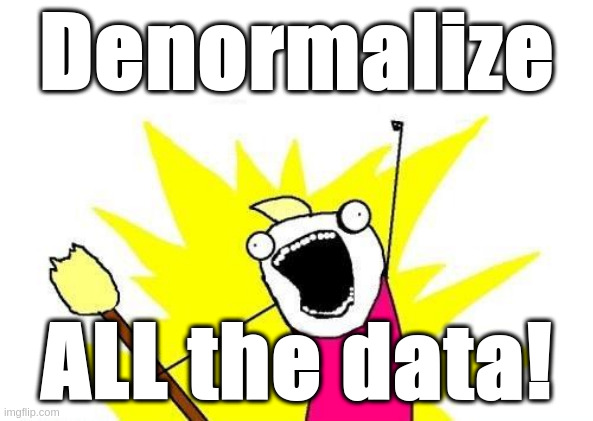
\includegraphics[width=0.4\textwidth]{images/denormalize.jpg}
\end{center}

 \end{frame}



\begin{frame}
\frametitle{NoSQL}


I sometimes have Fourth Year Design Project groups come to me and tell me they want to use NoSQL on a single user app that runs occasionally... 

Does that make sense?


\end{frame}



\begin{frame}
\frametitle{NoSQL = Speed!}

If you ask them their motivations, such students will say something along the lines of, NoSQL is faster. 


\begin{center}
	
\includegraphics[width=0.4\textwidth]{images/serious.png}
\end{center}

\end{frame}



\begin{frame}
\frametitle{NoSQL = Speed!}

As we will soon see, it can be... but nothing comes for free. 

In any case, how much any particular app needs speed is an open question. Speed isn't everything. 


\end{frame}


\begin{frame}
\frametitle{Relational Database vs NoSQL}

The right place to start is assuming you want a relational database, that is, a typical SQL based system. 

There are a lot of advantages to this and they tend to scale pretty well for a typical workload. 

We can scale them up and we can scale them out, as we have discussed in the distributed databases section. 

We might be willing to give up the advantages of the relational database because we, more or less, have no choice.


\end{frame}



\begin{frame}
\frametitle{NoSQL Motivation}

The primary motivation for wanting to go to NoSQL would likely be scalability. 

That is to say, storing very large amounts of data, handling heavy workloads, and making data accessible to users wherever they are. 

When we say a lot of data we're talking about things like Twitter, Facebook...

\end{frame}



\begin{frame}
\frametitle{Horizontal Scaling}

An upside of NoSQL databases is that they scale horizontally quite well. 

Unlike in SQL there is no need to do some magic to get a single server as big and fast as possible or to manually scale it across multiple servers. 

NoSQL, however, allows \alert{automatic sharding}: they natively and automatically spread data across an arbitrary number of servers.  


\end{frame}



\begin{frame}
\frametitle{Tradeoffs}

What we want to do is ultimately limited by the CAP theorem, also known as Brewer's theorem. 

There exists an iron triangle in distributed data stores.

 The CAP theorem says that it is impossible to get more than two out of the following guarantees: Consistency, Availability, Partition Tolerance.

\end{frame}



\begin{frame}
\frametitle{CAP Theorem}

Instead of 2 out of 3, it's choose either availability or consistency.

\begin{center}
	
\includegraphics[width=0.4\textwidth]{images/downtime.jpg}
\end{center}

This is because there \textit{will} be network failures or at least delays, meaning there is partitioning, even if it is temporary. 

\end{frame}



\begin{frame}
\frametitle{CAP Theorem}

\begin{center}
	\includegraphics[width=0.25\textwidth]{images/cap.jpg}
\end{center}

If reads can happen before all nodes are updated, we get availability. 

If systems require locking all nodes before allowing a read, we get consistency.

\end{frame}



\begin{frame}
\frametitle{Booking a Flight}

If we choose to prioritize consistency and there is network partitioning? 

Then we would refuse to allow any updates like seat selection until such time as all servers are in agreement and the seat can be locked on all nodes. 

If we choose availability, then in the event of partition we allow the person to choose the seat anyway, which may be based on stale data. 

In that case, you might have let two people choose the same seat and there will be a need to sort this out later. 

\end{frame}

\begin{frame}
\frametitle{Flying a Book}
For something like booking flights we might think it sensible to choose consistency over availability.

There is only one seat 32D on the airplane and it isn't exactly the same as any other seat. 

What if instead it was online shopping and you want to buy a book? 

One copy of the book is as good as any other, isn't it?

\end{frame}



\begin{frame}
\frametitle{I just wanted a sweater...}

I was looking to buy a shirt and sweater, both of which were listed on the website as being available in the colours and sizes that I wanted. 

After suffering through the checkout process I received an e-mail telling me that I had successfully placed the order and the items would be shipped. 

Then, a while later I received another e-mail telling me they don't actually have the items and can't ship them and they're really sorry. 

And their website still showed the items as available. 

\end{frame}



\begin{frame}
\frametitle{No ACID: BASE!}

For the most part, NoSQL databases do not provide ACID transactions. 

What you get is sometimes called BASE: Basically Available, Soft State, Eventually Consistent. 

The first two points are fairly obvious, but the new part in that acronym is \alert{eventual consistency}.

\end{frame}



\begin{frame}
\frametitle{Eventual Consistency}

This is to say that eventually, after some nontrivial period of time, the data will reach consistency. 

\begin{center}
	
\includegraphics[width=0.5\textwidth]{images/eventually.png}
\end{center}

If someone posts something you may not see it eventually as it could take some time for that thing to propagate its way through the network to you. 

\end{frame}



\begin{frame}
\frametitle{Eventual Consistency}


Now, the problem is you might never catch up, because the content is constantly being updated. 

People are posting new pictures of their dinner at every moment. 

It is not super important whether or not you learn whether your friend Terry ate that artisan heirloom radicchio.

\begin{center}
	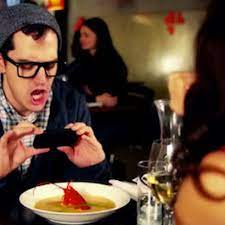
\includegraphics[width=0.3\textwidth]{images/eidti.jpg}
\end{center}

\end{frame}



\begin{frame}
\frametitle{Freeeeeeeedooooooommmmmm!}

As a developer it can feel like freedom to no longer have to worry about designing database tables, adding columns, and thinking about foreign keys. 

The rules are just slowing you down! 

\begin{center}
	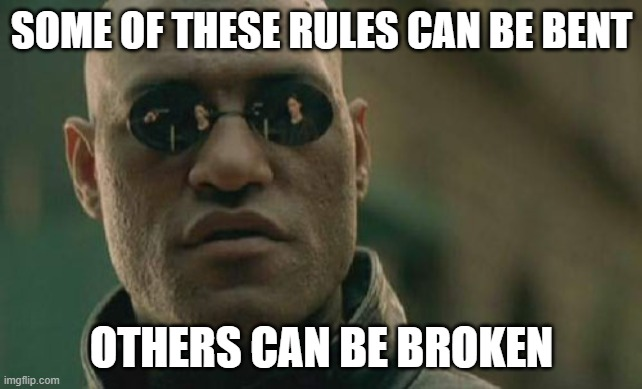
\includegraphics[width=0.5\textwidth]{images/breakrules.jpg}
\end{center}

\end{frame}



\begin{frame}
\frametitle{Freeeeeeeedooooooommmmmm!}

Making you do a bunch of boring stuff, forcing you to talk with a database administrator about adding a column here or changing a data representation... 

Although there are probably some rules in organizations that you can do without, there are reasons for some of them that are valid...

\end{frame}



\begin{frame}
\frametitle{Structure Can Be Good}

Structure standardizes data representation where possible. 

If there is an address table in the database and different developers want to use it in different scenarios, they can re-use the already existing structure.

You don't want three different address types, all subtly different.

\end{frame}



\begin{frame}
\frametitle{Structure Can Be Good}


Moreover, if you make some changes in a SQL database to a table you will need to think about the migration strategy.

In a relational database you're kind of forced to do this...

\end{frame}



\begin{frame}
\frametitle{Go Faster Through Lack of Safety}

Some of the NoSQL databases get speed by deleting some features that were very important throughout the course. 

There may be no joins. Really, no joins at all. 

\end{frame}



\begin{frame}
\frametitle{Go Faster Through Lack of Safety}

And why would there be if there are no tables and therefore no good ways to relate two data elements together? 

If there are no joins then related data has to be stored together, namely in de-normalized schemas.

Joins are slow so let's not have joins!

\end{frame}


\begin{frame}
\frametitle{Wait, we need those...}

Thing is, though, joins enforce consistency, so we might lose consistency in our database as a result of this. 

Duplicate data, or multiple entries of the same data that are all slightly different, any one of which you might get back in a particular query. 

For some things you may not care all that much. 

If it is something like keeping track of how many megabytes of data the user has used this month then ``close enough is good enough''... Maybe.


\end{frame}



\begin{frame}
\frametitle{NoSQL with Joins}

Some NoSQL implementations do allow joins but they don't work quite like your typical SQL join with join attributes defined in a query... 

You can, if you want, write your own sort of join, where you do some sequential lookup: first look up record $x$ which contains a way to find related record $y$...


\end{frame}



\begin{frame}
\frametitle{NoSQL with Joins}

 This might be acceptable for finding an individual record, but to do so for 10~000 records is tedious. 
 
 So perhaps you need to write your own join? At least we learned how those algorithms work... 

But why are you trying to reinvent the wheel?

\end{frame}



\begin{frame}
\frametitle{NoSQL NoTransactions}

Another way that NoSQL might work is it might not have transactions at all. 

Things happen, or don't, or might be halfway completed. 

It's up to you as the application developer to try to do things atomically or have some sort of failure recovery (rollback) mechanism. 

We'll consider, later, a case study about the Oracle NoSQL product that has something resembling a transaction.


\end{frame}



\begin{frame}
\frametitle{Types of NoSQL Database}

As you might already know, the variants of SQL that different databases speak can cause some problems.

You can't necessarily take a query written for MySQL and use it in Postgres.

It might be necessary to convert it because keywords are a little different.

Instead of working on the basis of relations with tables and keys and whatnot, how do NoSQL databases work?


\end{frame}


\begin{frame}
\frametitle{Types of NoSQL Database}

There's no simple, single answer to this because there are a lot of options. 

We'll look at: key-value databases, document databases, column databases, and graph databases.

\end{frame}



\begin{frame}
\frametitle{Types of NoSQL Database}

NoSQL tools do not have any sort of standardized language between them.

\begin{center}
	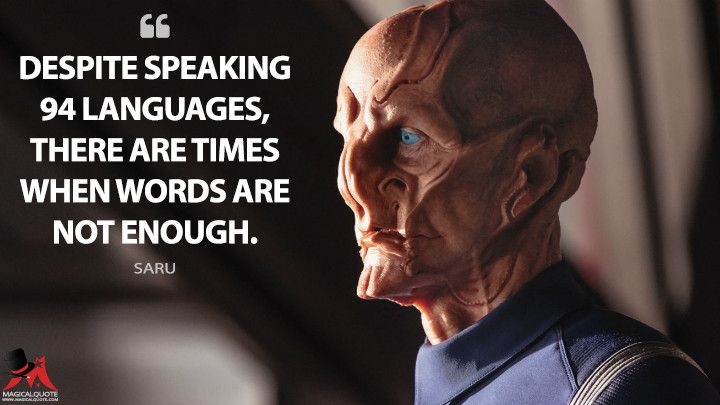
\includegraphics[width=0.7\textwidth]{images/saru.jpg}
\end{center}

Every vendor has their own idea about what's best and how things should work. 


\end{frame}



\begin{frame}
\frametitle{Key-Value Databases}

You are familiar with the idea of a key-value pair. 

In data structures and algorithms you learned about a Map (HashMap) for example that operates on the basis of \texttt{get( key )} and \texttt{put(key, value)}. 

Key-value pairs are a recommended way to store small amounts of data for things like Android applications. 

\end{frame}



\begin{frame}
\frametitle{Key-Value Databases}

Now that idea is applied to a larger amount of data. Instead of defined tables with specific attributes, you have an arbitrary key and an arbitrary value. 

There may be no restrictions on the form of the key or the form of the value.

This allows you to store anything you like... pdf documents, Java objects, flat text, comma-separated data... anything.


\end{frame}



\begin{frame}
\frametitle{Key-Value Databases}

This scales well, since the only operations are get (read) and put (write). 

There are no complexities related to searching, foreign keys, transaction management...

\end{frame}



\begin{frame}
\frametitle{Key-Value Databases}

Eventual consistency can be achieved when every location, sooner or later, gets the update of the data. 

Put operations simply overwrite old data, and data elements (values) have no formal relationships to one another. 

You can create some ad-hoc ones by storing under one key a list of other keys, but this is informal.


\end{frame}



\begin{frame}
\frametitle{Key-Value Databases}

Another thing that we don't get in this situation is aggregation or other ``magic'' the database can do for you. 

Remember that you can ask a relational database to sum a certain thing for you: how much income was generated in July of 2016? 

This is a select with aggregation and we can load just the data we need and crush it down to a single number (385~000) and transmit that result. 

\end{frame}



\begin{frame}
\frametitle{Key-Value Databases}

In a key-value store you have to do your own addition in application code. 

That itself isn't necessarily bad but your performance might be slow if you have to load a large amount of data from the database and send it to the application. 

\end{frame}


\begin{frame}
\frametitle{Column Databases}

Column databases are pretty much like key-value pairs with a slight bit of structure tacked on to the value part of it. 

A value has three components: name, the content (``value''), and a timestamp. 

The name is really the key; the value and timestamp are stored under that key.

\end{frame}


\begin{frame}
\frametitle{Column Databases}

 A column is then a logical view that encompasses, key, value, and timestamp all together. 
 
 The timestamp is used if we ever need to differentiate between different versions of the data and in case of recovery.


\end{frame}


\begin{frame}
\frametitle{Document Database}

A document oriented store is somewhat more structured than the simple key-value pair. 

Instead of just treating the value in they key-value pair as an opaque series of bytes, we might analyze it and do something with it. 

\end{frame}


\begin{frame}
\frametitle{Document Database}

\begin{center}
	
\includegraphics[width=0.4\textwidth]{images/folders.jpg}
\end{center}

Based on the structure of the value, as a document, it might be possible to extract some (meta)data about the document. 

Then we can use that for something else (e.g., search). 

\end{frame}



\begin{frame}
\frametitle{Document Databases}

We could store lots of documents in the database in formats like XML, JSON, or binary data like PDF or Word documents.

The documents themselves don't need to be formatted in any specific way.

The basic operations are generally defined as CRUD:

\textbf{C}reate (insert/put), \textbf{R}etrieve (query/search/get), \textbf{U}pdate (edit), \textbf{D}elete (remove).

\end{frame}



\begin{frame}
\frametitle{Document Database}

Aside from the convenience of CRUD rather than get/put, the major advantage is the analysis that allows searching or perhaps better query performance. 

If we wanted to search for documents with a certain element, e.g., find all documents relating to a particular Tax ID?

Having done the meta-analysis we could (maybe) find them relatively quickly if we have an index.

\end{frame}



\begin{frame}
\frametitle{Document Database}

\begin{center}
	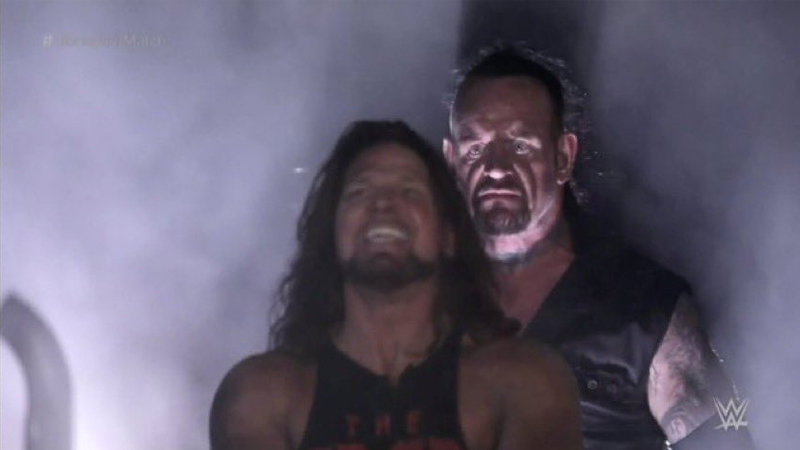
\includegraphics[width=0.5\textwidth]{images/undertaker.jpg}
\end{center}

Still, this can be a ``Data Grave...''

\end{frame}



\begin{frame}
\frametitle{Graph Databases}

In a graph database, a graph structure is used.

There are nodes, edges, and properties. 

Nodes and edges are first-class entities. 

\end{frame}



\begin{frame}
\frametitle{Graph Databases}


What we consider an entity in a relational database is modelled as a node. 

What is modelled as a relationship in the relational database is an edge. 

Nodes can have properties, and so can edges. 

This approach might even seem more natural for certain use cases than the standard relational model approach. 


\end{frame}



\begin{frame}
\frametitle{Graph Databases}

This supports a lot more ideas about joining, relationships, and constraints. 

It is still avoiding a lot of the structure imposed by the standard relational database.

In fact, we have something that looks like the document store model -- there are only two kinds of first-class elements (instead of everything being a table.  

But we don't necessarily give up the idea of formal relationships between entities.


\end{frame}



\begin{frame}
\frametitle{Example: Oracle NoSQL}

The Oracle NoSQL database provides something like transactions that are a practical approximation of ACID compliance. 

\begin{center}
	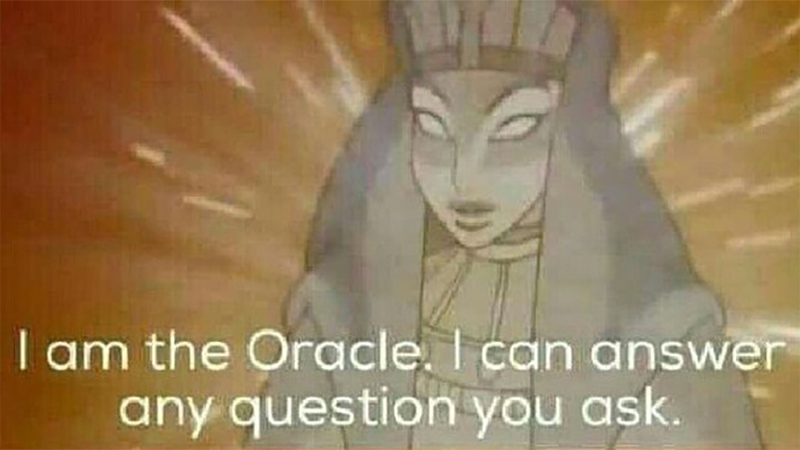
\includegraphics[width=0.35\textwidth]{images/oracle.jpg}
\end{center}

Instead of a simple key-value structure, Oracle divides the key into major and minor parts. 

The major is an object identifier and the minor parts are the ``fields'' in the record. 

\end{frame}


\begin{frame}
\frametitle{In the Key of C Major}

Instead of just the value as an impenetrable blob, it has an object with multiple fields and the names of those fields are now just called minor keys. 

So if a user has some unique ID and then associated things like addresses, the major key is the user ID and the minor keys are the address elements


\end{frame}




\begin{frame}
\frametitle{Or Maybe it's A Minor}

In short you get an ACID ``promise'' when all writes in a group are attached to the same major key. 

This makes it suitable for certain types of work: updating a user's personal information and storing it, for example. 

It is not suitable, however, for a standard bank example of transferring money from account $A$ to $B$. 

Because the transaction hits 2 separate accounts under 2 separate major keys. 

\end{frame}



\begin{frame}
\frametitle{Major and Minor Keys}

One master machine is guaranteed to hold all minor keys associated with a major key.

All these minor attributes are on the same node and we can therefore get consistent behaviour through the use of local locks and it all works. 
 
But no such guarantee is provided for when the major keys are different because they could be located on different nodes. 
 
They might be on the same node and things might work, but there are no promises. 

\end{frame}



\begin{frame}
\frametitle{Scaling Oracle NoSQL}

Oracle NoSQL offers both kinds of scaling, replication and sharding. 

With sharding, your data is spread out and you have less contention (faster writes). 

If you have replication you get faster reads and higher availability of data (and reliability in some sense). 

Of course, the more replication you have the longer it can take to write some data, because you do have to get all the systems to agree. 

\end{frame}



\begin{frame}
\frametitle{Durability Policy}

But even that is configurable: you can tell the system what ``durability policy'' you want to have. 

Choose if writing successfully to one node enough, or if a simple majority is sufficient, or if all nodes need to agree on the write. 

Values are associated with a version number which you can use in writing your own sort of replication and durability policy if you so desire

\end{frame}



\begin{frame}
\frametitle{NoSQL: Conclusions}

NoSQL has lots of advantages and disadvantages when compared to standard relational databases. 

If used in the right situation, it can speed operations and provide a lot of scalability and availability.

 If used in the wrong situation it either wrecks your application/company, causes endless headaches, or forces you to reinvent the wheel.
 
 \end{frame}



\begin{frame}
\frametitle{NoSQL: Conclusions}

 
 Start with the idea of using a relational database, and consider carefully what you would be losing if you went to a NoSQL approach.
 
  If it's the right call for this need, then, by all means. You have the power and the choice is yours. Choose wisely.


\end{frame}




\end{document}

